\subsection{Overview}\label{subsec:overview}
\paragraph{}
An alternative to the security patch it would also be possible to re-write the entire application to not only remedy the addressed
security issues but also make improvements to a few key traits.

\subsubsection{Core Requirements}\label{subsubsec:core-goals}
\paragraph{}
There are few core requirements that are the pillars of the application.
Again they are only touched upon for brevity, thus I would be happy to explain them further at request.

\paragraph{Offline First (PWA) - \emph{Optional}}\label{para:pwa}
Unfortunately it would be unrealistic to assume that the mobile users of the application would have a good connection to the internet at all times.
Whether it is a job in a location where reception is not reliable or a network outage the application would need to handle situations where
it expects to not have instantaneous access to a server.
This is where \href{https://web.dev/progressive-web-apps/}{\textbf{Progression Web Apps (PWA's)}} strive.
It is important to note that functionality would be limited whilst offline leading to an increased development cost.
As a result I have separately quoted this feature.

\paragraph{Limited Data Transfers}
As the application UI would be a single page application we can limit the data transferred from the server.
There would be an increased load time for the initial application to download the static assets and general UI that is then cached for
later use.
With that in place the only data required from the server would be dynamic data such as user jobs.
This data would be transferred in a minimal format such as JSON in which the application would render suitable components.

\paragraph{Purpose Driven UI Navigation}
As there is a varied user base it is important for functionality to be clear and flow in a way that allows the user
to achieve what they need naturally without the need to translate the real life task into the applications' workflow.
\begin{description}
    \item \emph{Limit Paths:} Although it may sound counter-intuitive it is important to limit the paths that a user can take through
    an application.
    This not only makes the process clear for the user but also gives management an easy measure to reflect the correct process.
    \item \emph{Relevant Elements and Reducing Page Jumps:} It is important that elements and information required for tasks is presented or easily accessible to the user.

    \item \emph{Mobile Friendly:} As the majority of users would be using a mobile device it is important that the application is optimised
    to be used on mobile devices.
\end{description}

For a clear example it would be worth looking at the prototype page \href{https://cpr.caleb-dunn.tech/jsheet/5116}{\textbf{HERE}}.

\paragraph{Resource Efficient and Scalable}
It is ultimately the goal of any software to be resource efficient, fast and scalable but to achieve this the software architecture must be
thoughtfully planned out.
By using appropriate and fast technologies / languages for certain sections of the application allow for using the right tool for the job.
The proposed design aims to separate layers of the application that would allow for more instances to be spun up although this would
likely not be needed due to the scope of the application.

\paragraph{Native Application Potential}
Whilst a native mobile application is not included in the software package it would be possible to implement a technology like \href{https://reactnative.dev/}{\textbf{React Native}} to
develop a native mobile application that could be installed onto devices whilst leveraging the existing code for the website.
This would be more robust than the \hyperref[para:pwa]{\textbf{PWA}} but would require more development.

\subsubsection{General Application Flow}
\paragraph{}
Below is an example of how a user authenticates and interacts with the application and how the components interact with each other.

\paragraph{Assumption}
User has an account and has already visited the website and downloaded required assets.
\begin{enumerate}
    \item User Login
    \begin{enumerate}
        \item User enters login credentials on login page.
        \item Credentials are sent to GO webserver through Caddy proxy.
        \item GO webserver retrieves user details from PostgreSQL matched on username.
        \item Compute password hash for password sent to server and compare with the existing stored hash. \emph{If invalid user is notified and re-prompted to login.}
        \item Generate and set access token for user session in Redis and as a client cookie.
    \end{enumerate}
    \item User navigates to current jobs.
    \begin{enumerate}
        \item Using access token in cookie a request is sent to the webserver.
        \item The webserver uses the access token to retrieve the user session from Redis.
        \item If the access token and user session is valid the webserver requests the users job data from PostgreSQL.
        \item Webserver serialises jobs into JSON and sends back to user.
        \item User receives jobs to interact with.
    \end{enumerate}
\end{enumerate}


\pagebreak

\subsubsection{General Data Request Example}
\paragraph{}

\begin{figure}[h!]
    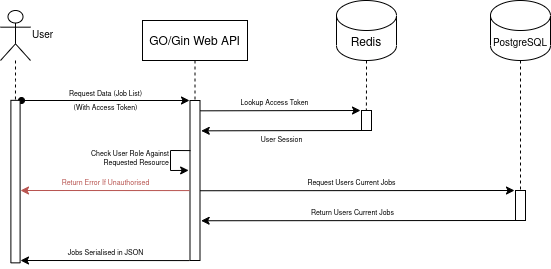
\includegraphics[width=\textwidth]{res/general-api-request}
    \caption{A generic job data retrieval}
    \label{fig:general-api-req}
\end{figure}

\pagebreak
\subsection{Major Components}\label{subsec:major-components}
\subsubsection{GO Gin REST API}

\paragraph{GO Summary}
GO is a modern compiled language created by Google with the purpose of being simple and easy to learn with a strong concurrency model.
This purpose fulfils CPR's requirements with its backend service as it's simplicity allows for ad-hoc future development and by nature web services
are concurrent in nature serving multiple users at a given time.

\paragraph{} GO Documentation: \url{https://go.dev/doc/}

\paragraph{Gin Summary}
Gin is a HTTP framework that abstracts away from lower level \href{https://pkg.go.dev/net/http}{http} package leading to a monumental decrease
in complexity and development time.
Gin leverages of GO's goroutines to serve each request concurrently whilst maintaining the simplicity of single threaded programming.

\paragraph{} Gin Documentation: \url{https://github.com/gin-gonic/gin}


\subsubsection{ReactJS Front End}

\subsubsection{Caddy Webserver}
\subsubsection{PostgreSQL Database}
\subsubsection{Redis Session Cache}

\subsection{Advantages vs Current System}\label{subsec:advantages-vs-current-system}

\subsection{Advantages vs Implementing Security in Existing System}\label{subsec:advantages-vs-implementing-security-in-existing-system}
\clearpage
\printglossaries